\documentclass[10pt,letterpaper,twocolumn]{article}

\usepackage[top=2.1cm,left=2.0cm,right=2.0cm,footskip=2.0cm]{geometry}
\usepackage[utf8]{inputenc}     % for Unicode
\usepackage{cite}               % citation
\usepackage[dvipdfmx]{hyperref} % links
\usepackage{caption}            % caption
\usepackage{microtype}          % improves typesetting in LaTeX
\usepackage{algpseudocode}
\usepackage{algorithm}
\usepackage{graphicx}
\usepackage{color} % ex.) \textcolor{color}{text}
\usepackage{url}

\renewcommand{\algorithmicrequire}{\textbf{Input:}}
\renewcommand{\algorithmicensure}{\textbf{Output:}}

\setcounter{topnumber}{3}
\setcounter{dbltopnumber}{6}
\renewcommand\topfraction{.9}
\renewcommand\textfraction{.1}
\renewcommand\dbltopfraction{.9}
\renewcommand\dblfloatpagefraction{.9}

\begin{document}

\twocolumn[
    \begin{flushleft}
        {\Large
        \textbf\newline{
            Periortree: An Extention of R-Tree for Periodic Boundary Conditions
            }
        }
        \newline
        \\
        Toru Niina \textsuperscript{1}
        \\
        \bigskip
        \bf{1.} Department of Biophysics, Graduate School of Science,
                Kyoto University, Kyoto 606-8502, Japan
        \\
        \bigskip
        * niina@theory.biophys.kyoto-u.ac.jp
    \end{flushleft}

    \section*{Abstract}
    Searching spatial data is an important operation for scientific simulations
    which are performed mostly on periodic boundary conditions.
    An R-Tree is a widely used tree data structure used to contain spatial
    objects and it is capable of answering to spatial searching queries in an
    efficient way.
    In this paper, A novel method to construct R-Tree considering periodic
    boundary conditions is introduced.
    Unlike existing methods, this method works without any kind of additional
    set of objects or queries.
    Moreover, because this method reduces the size of bounding boxes for each
    nodes under the periodic boundary conditions, it is expected to increase
    the efficiency.
    This method is essentially applicable not only to the Guttman's original
    R-Tree but also to other data structures that use axis-aligned bounding
    boxes.
    The implementation is available on GitHub.
    \bigskip
]

\section*{Introduction}

Computational simulations are essential tools for scientific research, such as
investigating behaviors of complex biochemical models. To perform such large
scale simulations, both huge amount of computational resources and efficient
simulation softwares are required.

In most cases, searching for objects that satisfy some geometrical conditions
is one of the most time-consuming operation in a simulation. Generally, an
efficient algorithm that search spatial objects drastically accelerates not only
the whole simulation processes, but also the data analysis of simulation results.
Therefore, a method that efficiently processes spatial search accelerates the
whole process of scientific simulation research.

An R-Tree is a widely used data structure representing bounding volume
hierarchies (BVH) by using an axis-aligned bounding box (AABB) for all its
entries \cite{Guttman1984}.
It is capable of containing both sizeless and finite sized objects such as
points, segments, rectangles, spheres, etc.
In order to improve the efficiency or to extend it to be able to store the
different kind of the objects, many variants of R-Tree have been proposed.
\cite{Beckmann1990, Leuteneggert1997, Berchtold2001, CoSTR-R-tree2016}.

In order to use an R-Tree with periodic boundary conditions (PBCs), currently,
two methods have been proposed (figure\ref{fig-method-rtree-pbc})
\cite{CoSTR-R-tree2016}.
The first method is described in figure \ref{fig-method-rtree-pbc}A.
It stores all the possible periodic images of the simulation system.
Because the periodic images exists explicitly, it enables an R-Tree to
contain and search objects considering PBCs.
However, it consumes memory $3^D$ fold (where $D$ reprecents a dimension of a
system) relative to the memory consumption of a normal R-Tree.
The other method (figure \ref{fig-method-rtree-pbc}B) does not store the
periodic images.
When the query sticks out of the boundary, it replicates the query based on the
PBCs by transposing it periodically.
Although it works fine with points, it has a limitation when working with
finite-sized objects. It might overlook objects if query is inside of
the boundary and objects extend beyond the unit cell
(figure\ref{fig-method-rtree-pbc}C).
One ad-hoc solution to overcome this limitation is changing the criteria to
replicate a query based on the elements that is contained.
This may increase the frequency of copying queries and decrease the efficiency.

Here a novel method to construct and use an R-Tree under the PBCs is proposed.
The main idea is to consider the PBCs in each step to insert entries to an
R-Tree and search objects in an R-Tree.
By expanding an AABB corresponding to each node along the boundary conditions,
an R-Tree becomes capable of containing objects in the most intuitive way and
overcomes the limitation of containing finite-sized object under the PBCs
(figure\ref{fig-method-rtree-pbc}D).

In the method part, It is shown that most of the operations such as intersection
detection can be implemented just by introducing periodic transpose to the
algorithms when one use the appropreate representation of an AABB.
Consequently, this method require the specific representation or
conversion between the representations of an AABB.

This method does not require to copy objects or queries.
Moreover, using the information of the boundary condition, it has more chance
to reduce the volume of AABBs of each node. Since the efficiency of spatial
searching with an R-Tree is strongly affected by the size of each nodes,
in most cases, this feature has possibility to increase the efficiency of
spatial searching.

\begin{figure}[hbt]
    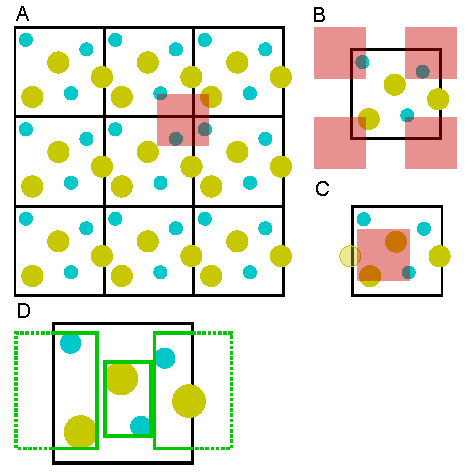
\includegraphics[width=8.4cm, bb=6 3 220 224]{fig1.eps}
    \caption{Methods to handle R-Tree on periodic boundary conditions.
    (\textbf{A})
    By copying the unit cell for each dimension along periodicity, normal R-Tree
    can manage objects that are associated with periodic images.
    (\textbf{B})
    By adding extensional query translated for each periodic images, R-Tree can
    detect objects that are beyond boundary.
    (\textbf{C})
    With the method described in \textbf{B}, finite sized objects could be
    overlooked when queries that is inside of the boundary are not copied.
    (\textbf{D})
    This is the method proposed in this paper. Forming rectangles according to
    the periodicity, R-Tree can organize objects on periodic boundary
    conditions.}
    \label{fig-method-rtree-pbc}
\end{figure}

The codes that are used for this paper is available on GitHub
(\url{http://github.com/ToruNiina/periortree}).

\section*{Methods}

Here some operations to modify and handle rectangles under PBCs are introduced.
The algorithm to grow and maintain an R-Tree is not modified at all.
Hence, in this section, the algorithm to construct and maintain R-Tree itself is
not explained.
The fact that this method is independent from an R-Tree algorithm means that
the method can be applied to R-Tree variants and other spatial indexing
methods that are baded on BVH and AABBs.

Because the rectangles used in R-Tree are axis-aligned, it is sufficient to show
an operation for one dimension to provide the whole algorithm. Applying it to
each dimension successively, these operations can be extended for higher
dimension cases.

\paragraph{Representation of PBCs.}
Here, as the unit cell of the PBCs, only cuboids are considered.
All the coordinates of the objects are assumed to be restricted to be inside of
the unit cell.
There are well-known algorithm to restrict coordinates and inter-position
vectors to the unit cell.
In this paper, these algorithms are called as \textbf{RestrictPosition} and
\textbf{RestrictVector}, respectively.

\paragraph{Representation of AABBs.}
There are three common representations for AABBs
(figure~\ref{fig-rectangle-rep})~\cite{real-time-collision-detection}.
The first one is a pair of the minimum and maximum coordinate values
in each dimension.
The second one is a pair of the minimum coordinate values and its width in each
dimension.
The third one is a pair of the center position and half-width in each dimension.
Here, these are called as min-max, min-widths, and center-radius representation,
respectively.

Because the method proposed in this paper uses a center position of an AABB
quite often, here center-radius representation is employed.
\begin{eqnarray}
    rectangle = \{center, radius\} \nonumber
\end{eqnarray}
The center-radius representation makes the implementation simple, but it is not indispensable.
Because all the representations have identical information about an AABB,
one can convert one representation to another.

\begin{figure}[thb]
    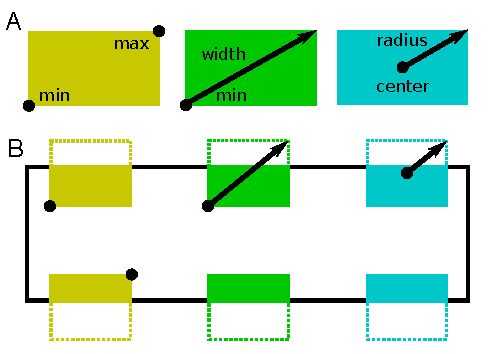
\includegraphics[width=8.4cm, bb=2 6 226 165]{fig-rect-rep.eps}
    \caption{
    (\textbf{A})
    Three popular representations of an AABB. The first one is min-max,
    the second one is min-widths, and the third one is center-radius representation,
    respectively.
    (\textbf{B})
    Three representations on PBCs.
    The AABBs are colored in the same way as \textbf{A}.
    }
    \label{fig-rectangle-rep}
\end{figure}

\paragraph{Expanding AABBs according to PBCs.}
Expanding an AABB to ensure it contains a new object is one of the most
important operations in an R-Tree algorithm.
Because the total area that is covered by AABBs in the nodes of an R-Tree
affects the efficiency of spatial searching, it is needed to find the way to
make the area of the rectangle in each node as small as possible.

The algorithm to find the minimum expansion of AABB to contain another AABB on
PBCs is shown in algorithm ~\ref{expand_aabb_aabb}.
The size of a bounding box that contains two rectangles is determined by the
distance between center points of the contents and the radius of the contents.
Therefore, by finding the minimum distance between the center points of the contents, the minimum expansion can be found. To minimize the distance between two points on PBCs,
the \textbf{RestrictVector} can be used.

For the case of containing points, it becomes simpler as described in the algorithm
~\ref{expand_aabb_point}.
Just by finding the minimum distance between the points to be contained, the minimum expansion can be found.

\begin{algorithm}[thb]
    \caption{expand AABB so that it contains another AABB}
    \label{expand_aabb_aabb}
    \begin{algorithmic}
        \State $R1 \gets$ AABB to be expanded
        \State $R2 \gets$ rectangle to be contained
        \State $B  \gets$ boundary
        \Function{ExpandAABB}{$R1, R2, B$}
            \State $dc \gets R2.center - R1.center$
            \State $dc \gets$ \Call{RestrictVector}{dc, B}

            \State $l1 \gets R1.center - R1.radius$
            \State $u1 \gets R1.center + R1.radius$
            \State $l2 \gets (R1.center + dc) - R2.radius$
            \State $u2 \gets (R1.center + dc) + R2.radius$

            \State $L  \gets \Call{min}{l1, l2}$
            \State $U  \gets \Call{max}{u1, u2}$
            \State $C  \gets (L + U) / 2$
            \State $HW \gets (U - L) / 2$
            \State $C  \gets$ \Call{RestrictPosition}{C, B}

            \State \Return $\{C, HW\}$
        \EndFunction
     \end{algorithmic}
\end{algorithm}

\begin{algorithm}[thb]
    \caption{expand AABB so that it contains a point}
    \label{expand_aabb_point}
    \begin{algorithmic}
        \State $R \gets$ AABB to be expanded
        \State $P \gets$ point to be contained
        \State $B \gets$ boundary
        \Function{ExpandAABB}{$R, P, B$}
            \State $dc \gets P - R.center$
            \State $dc \gets$ \Call{RestrictVector}{dc, B}

            \State $l \gets R.center - R.radius$
            \State $u \gets R.center + R.radius$

            \State $L  \gets \Call{min}{l, P}$
            \State $U  \gets \Call{max}{u, P}$
            \State $C  \gets (L + U) / 2$
            \State $HW \gets (U - L) / 2$

            \State $C \gets$ \Call{RestrictPosition}{C, B}
            \State \Return $\{C, HW\}$
        \EndFunction
     \end{algorithmic}
\end{algorithm}



\paragraph{Detecting an object includes or intersects the other object}

To find an object in an R-Tree, the algorithm is needed to check whether a
rectangle intersects or be inside of another rectangle.
It also can be determined by using the minimum distance between centroids of the
rectangles.
The existing algorithm for the center-radius representation can be applied after
restricting the vector between the center points of the rectangles.

\begin{algorithm}[tbh]
    \caption{Check whether an AABB is inside of an AABB}
    \begin{algorithmic}
        \State $R1 \gets$ rectangle
        \State $R2 \gets$ rectangle that might be inside of R1
        \State $B  \gets$ boundary
        \Function{IsAABBInsideOfAABB}{$R1, R2, B$}
            \State $dc \gets R1.center - R2.center$
            \State $dc \gets$ \Call{RestrictVector}{dc, B}

            \State \Return \Call{abs}{dc} $\leq (R1.radius - R2.radius)$
        \EndFunction
     \end{algorithmic}
\end{algorithm}

\begin{algorithm}[tbh]
    \caption{Check whether a point is inside of an AABB}
    \begin{algorithmic}
        \State $R \gets$ rectangle
        \State $P \gets$ point that might be inside of R
        \State $B \gets$ boundary
        \Function{IsPointInsideOfAABB}{$R, P, B$}
            \State $dc \gets R.center - P$
            \State $dc \gets$ \Call{RestrictVector}{dc, B}
            \State \Return \Call{abs}{dc} $\leq R.radius$
        \EndFunction
     \end{algorithmic}
\end{algorithm}

\begin{algorithm}[tbh]
    \caption{Check whether an AABB intersects to another AABB}
    \begin{algorithmic}
        \State $R1 \gets$ rectangle
        \State $R2 \gets$ rectangle that might intersect to R1
        \State $B  \gets$ boundary
        \Function{IntersectsAABB}{$R1, R2, B$}
            \State $dc \gets R.center - R.center$
            \State $dc \gets$ \Call{RestrictVector}{dc, B}
            \State \Return \Call{abs}{dc} $\leq (R1.radius + R2.radius)$
        \EndFunction
     \end{algorithmic}
\end{algorithm}

\section*{Results}


The three steps of expansion of an AABB to contain rectangles is shown in
figure~\ref{fig-result}A. In the figure, the objects to be contained are colored
in black, and the AABB containing its objects are colored in red.
While each figure shows several boxes, there is only one bounding box.
Because it sticks out of the boundaries, the periodic images of the bounding box
are shown separately.
The last panel in figure~\ref{fig-result}A shows that the method successfully
found the way to expand AABB with the least enlargement. Clearly, if the AABB
expanded independently from the PBCs, the AABB would wrap most of the area of
the system.

In figure~\ref{fig-result}B the result of a query is shown. It successfully
detects an object that locates beyond the boundaries. It should be noted that
while there are four query-rectangles drawn in the second panel of figure
~\ref{fig-result}B, actually there is only one query-rectangle.

\begin{figure}[htb]
    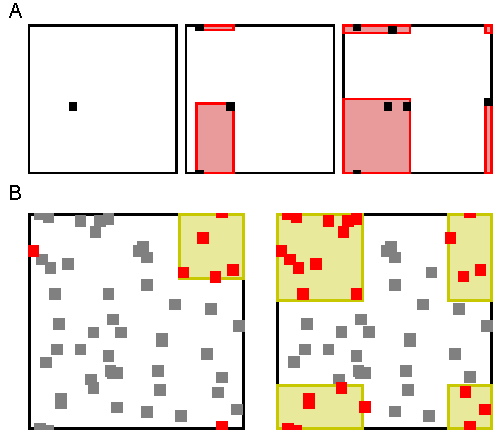
\includegraphics[width=8.4cm, bb=4 6 237 212]{fig-result-expand-intersect.eps}
    \caption{
    (\textbf{A})
    The three steps to expand AABB colored in red to contain black rectangles.
    It can be seen that the AABB are expanded beyond the boundary.
    (\textbf{B})
    The result of querying objects that intersect to yellow rectangle.
    The object contained in the R-Tree is shown as small square boxes.
    The boxes that are detected as intersecting to the query rectangle is
    colored in red.
    }
    \label{fig-result}
\end{figure}

\section*{Conclusion}

In this paper, the novel method of applying PBCs to R-Trees is introduced.
To detect some kind of geometrical condition such as intersection, the existing
method can be used after periodic transpose when the AABBs are represented
in center-radius representation.

The method proposed in this paper is capable of containing not only sizeless points but also finite-sized objects. The method can remove the necessity of both storing extensional objects or replicating queries. Moreover, it reduces the
size of each node based on the PBCs.

On the other hand, the method introduces tiny but unavoidable computational
costs into each procedure for maintaining R-Tree and checking geometrical
conditions. It considers the boundary condition for all of the recursive steps
to find objects in nodes and all of the steps to contain new objects.

As described before, since the method is only for modifying and handling
rectangles on PBCs, it is essentially applicable for the other R-Tree variants
or the other kind of spatial indexing methods.

Because the adaptation of spatial indexing to a system on PBCs has a chance to
accelerate many kinds of scientific simulations, it is expected that this novel
method will have an important role for the simulations that will be performed in
the next decade.

\bibliographystyle{unsrt}
\bibliography{library}{}


% -> appendix
% Algorithm\ref{center_aabb} and \ref{radius_aabb} provide ways to convert the
% min-max representation to the center-radius representation according to the PBCs.
% It should be noted that the maximum coordinate value of an AABB might be smaller
% than the corresponding minimum coordinate value because all the coordinates are
% restricted to the inside of the unit cell by periodic transposing.
% It means that the AABB sticks out of the boundary.
%
% \begin{algorithm}[htb]
%     \caption{calculate the centroid of an AABB on PBCs.}
%     \label{center_aabb}
%     \begin{algorithmic}
%         \State $U \gets$ maximum coordinate values of an AABB
%         \State $L \gets$ minimum coordinate values of an AABB
%         \State $B \gets$ the unit cell of a boundary
%         \Function{CentroidAABB}{$U, L, B$}
%             \If{$U < L$}
%                 \State $C \gets (U + B.width + L) / 2$
%             \Else
%                 \State $C \gets (U + L) / 2$
%             \EndIf
%             \State \Return $C$
%         \EndFunction
%      \end{algorithmic}
% \end{algorithm}
%
% \begin{algorithm}[htb]
%     \caption{calculate the width of an AABB on PBCs.}
%     \label{radius_aabb}
%     \begin{algorithmic}
%         \State $U \gets$ maximum coordinate values of an AABB
%         \State $L \gets$ minimum coordinate values of an AABB
%         \State $B \gets$ the unit cell of a boundary
%         \Function{WidthAABB}{$U, L, B$}
%             \If{$U < L$}
%                 \State $W \gets U + B.width - L$
%             \Else
%                 \State $W \gets U - L$
%             \EndIf
%             \State \Return $W$
%         \EndFunction
%      \end{algorithmic}
% \end{algorithm}



\end{document}
